\def\bibliocommand{\bibliography{bibliography}}
\input{latBegin.txt}

\part{Introduction}
\label{introduction}

\chapter{Our closest cousins}
\label{ourclosestcousins}

The kingdom Fungi is one of the most diverse groups of organisms on Earth, and they are integral ecosystem agents with a huge impact on biogeochemical cycles, plant and animal pathology, plant nutrition and soil properties.
While historically clustered together with plants ~\citep{copeland1938, copeland1956}, towards the middle of last century it started to become clear that this lumping failed to properly deal with the differences between the two groups. In 1969 R. H. Whittaker published a paper dividing the organisms into five kingdoms: Animalia, Plantae, Fungi, Protista and Monera ~\citep{whittaker1969}. By the 70s this division became widely accepted, and the Kingdom Fungi was recognized.
Acknowledgement is just the first step in knowledge though. The understanding of the taxonomy, evolution and phylogenesis of fungi was still a matter of ample debate, one of those that may never end for lack of evidence. All the analysis were based on morphological differences, with all of its downsides.

Fossilized fungi are very difficult to come by, as they do not biomineralize like animals do, and has proven not only inconclusive with regard to the origin of fungi, but also rather incomplete relative to the evolutionary history of the various fungal lineages. The earliest compendium of fossil fungi is from the late 19th century ~\citep{meschinelli1898}, and the symbiotic relationship with plants in fossils was suggested around that period ~\citep{renault1896}, but the difficulty in the interpretation of morphological data made it impossible to actually understand what happened.

Earliest fossil with the morphological features of a fungus is dated to around 1 billion years ago, and was found in the Arctic Canada ~\citep{loron2019}, and there is evidence of fungus-like organisms in fossils of around 800 Mya ~\citep{bonneville2020}. Those findings are rare though, we surely have a richer diversity of fossils from the lower Devonian (around 400 Mya).

It wasn't until the large scale advent of molecular phylogenetics techniques that some light could be properly shed on the history of fungi ~\citep{james2006}.
From molecular clock analysis seems like fungi are sister group to animals, that is, the two lineages are close, diverging around 1.5 Billion years ago ~\citep{wang1999}. The two groups form one supergroup called Opisthokhonta ~\citep{cavalier-smith1987}, from the Greek opísthios (rear, posterior) and kontós (``pole'' i.e. ``flagellum''), since the group is characterized by flagellate cells that propel themselves with a single, posterior flagellum (in many cases lost).

IMG OF TREE WITH ANIMALS AND FUNGI AND PLANTS

\chapter{Ancient lovers}
\label{ancientlovers}

So: fungi are animals' cousins, and the two lineage diverged around 1.5 billion years ago. What happened then?

The ancestors of fungi are believed to be simple aquatic forms with flagellated spores, similar to members of the extant phylum Chytridiomycota (chytrids), which are now considered one of the early-diverging clade in the kingdom ~\citep{james2006}. The first terrestrial fungi colonized land probably before plants did ~\citep{heckman2001}, as saprobe (taking nutrition out of dead matter) and\slash or in symbiosis with organisms capable of photosynthesis.
It is commonly accepted that in order to colonize the land, plants had to develop a symbiotic relationship with fungi ~\citep{selosse1998, heckman2001, bonneville2020}, but it is not entirely clear whether this relationship was lichen-like or mycorrhizal-like.

IMG LICHEN

Lichens are the symbiotic relationship between a singol or more fungi (\emph{mycobiont})and a cyanobacteria or algae (\emph{photobyont}). Think about an algae floating in water: for many reasons, it is not really equipped to deal with the challenges of a terrestrial life style: mainly, it won't be able to mine substrate resources, to protect itself against dehydration, constant direct UV radiations and strong temperature fluctuations ~\citep{selosse1998, blackwell2000}. In a lichen, the photobiont is protected by the fungal stroma, and it can tolerate drought, cold, heat, intense light and barren rocky substrates. They also seem to be the first pioneers in a barren environment today, so everything would point to them being the right candidate for a first out-of-water plant-fungi symbiosis.

Yet, while this relationship evolved several times ~\citep{gargas1995}, the only phyla we know that are capable of such process (called \emph{lichenization}) are Ascomycota and, secondarly and later in time, Basidiomycota, and we can date the origin of those clades to about 400 Mya in the Devonian ~\citep{berbee1993}. Similarly we have fossils for lichens dating at the oldest in the Early Devonian (400 Mya) ~\citep{taylor1997, honegger2013}, while the first fossil land plants and fungi appeared 480 to 460 Mya, and molecular clock estimates suggests about 600--700 Mya ~\citep{berbee1993, heckman2001}.

Therefore, lichens were likely not what opened the way to plants for land colonization. Let's look now at a mycorrhizal-like relationship.

Mycorrhiza is the symbiotic association between plants and fungi happening in the rhizosphere, that is, the plant's root system. It consist in an exchange of resources between the fungus and the plant, ideally the plant providing sugar to the fungus and the fungus providing minerals and nutrients to the plant, even though it's hard to pinpoint who's benefiting who and it may fall on different scales of the parasithic-mutualistic spectrum

What we know is that fossils resembling mycorrhizal relationships have fossil dating back to the Ordovician (with an age of about 460 million years), and are Glomales-like Arbuscular Mychorrhizal (AM hereafter) fungi, in a moment where the land flora is supposed to only consist of plants on the bryophitic level ~\citep{redecker2000}. Now, plants can photosynthetize; these fungi can extract minerals from the substrate with great efficiency, protect the root system, extend the range from which water can be taken and protect the plants from pathogens. It's easy to see how this is going to end up in a passionate love story.

You could say ``\emph{wait a minute: those plants did not have true roots, how can we have a mycorrhizal relationship?}''. Good point. Fossil records provides evidence that fungal organisms entered in such symbiosis before the appearance of true roots, and as long as there is a multicellular host AM fungi are fine ~\citep{wang2006, bonfante2008}.

Whether as lichen or as mycorrhiza, the symbiosis between plants and fungi is one of the most important, most ancient relationship in the history of living beings and it surely played a crucial role in the successful colonization of the land by plants ~\citep{pirozynski1975, malloch1980, harley1987, trappe1987, selosse1998, brundrett2002}. The relationship is so beneficial (for one or both parts) that today is the norm, and is well established in c. 85\% of extant plants ~\citep{cairney2000, strullu-derrien2018}, with a high degree of complexity ~\citep{heijden2015}.

\chapter{Orchids}
\label{orchids}

Let's move the camera away from fungi for a second. Don't worry, we'll get back to them soon enough, but now we need to introduce the second protagonist of the present work: orchids.
Orchids are a diverse and widespread family of flowering plants, counting over 28,000 species in about 736 genera ~\citep{christenhusz2016}, second only to \emph{asteraceae} in terms of number even though they got on the scene only around 80 Mya ~\citep{ramirez2007}, not very long ago. They are cosmopolitan, with a distribution spanning all continents except Antarctica and including most major island groups ~\citep{givnish2016}.
By the end of 2017 the IUCN Global Red List included assessments for 948 orchid species, of which 56.5\% are threatened ~\citep{fay2018}. In Europe all wild orchids are protected, being included in their entirety on Appendices I and II of the Convention on International Trade in Endangered Species of Wild Fauna and Flora ~\citep{CITES-1} as are many of the habitats they live in, and are in many countries Red List. Nonetheless, this protection has not staved off a general decline in the orchid flora of Europe ~\citep{jacquemyn2005, kull2006}. Major threats include habitat destruction and unsustainable (often illegal) harvesting, and because of their complex life histories orchids are thought to be particularly vulnerable to the effects of global environmental change ~\citep{kull2016, gale2018}

Orchids exhibit an astonishing diversity of habitat adaptations, morphologies and pollination strategies, but some characteristics are common to the whole family. One of the most important is the reliance on Orchid Mycorrhizal Fungi (OMF hereafter) for reproduction and often outright survival. I told you we would soon get back to them.
Orchids seeds are devoid of nutritional resources, and they completely rely on fungi for nutrition including water, minerals and carbon supply ~\citep{leake1994, rasmussen1998, merckx2013} in a nutritional strategy called ``mycoheterotrophy''. After germination, seedlings often become autotrophic and subsequently revert to usual mycorrhizal functioning ~\citep{rasmussen1995, cameron2008}. Some species, especially from forest environments, remain mycoheterotrophic at adulthood though, developing partial photosynthetic capacity but still relying on fungi for carbon resources, a nutritional strategy called ``mixotrophy'' or ``partial mycoheterotrophy'' ~\citep{gebauer2003, julou2005, selosse2009}. Others never develop photosynthetic capacity and therefore rely completely on fungi for nutrition. This nutritional mode, which has evolved over 30 times independently in orchids, is called ``obligate mycoheterootrophy'' ~\citep{merckx2013}. So: no OMFs, no orchids.

While the relationship between orchids and OMFs is known since over a century ~\citep{bernard1899, rayner1927, rasmussen2002, selosse2011} and the mechanisms of this symbiosis are beginning to be properly understood, the knowledge from a taxonomical standpoint is still in full evolution. For many years orchids were thought to interact almost entirely with the members of the \emph{Rhizoctonia} complex. It was later discovered not only that orchids have way more interactions with different fungi also from the \emph{Ascomycetes} phylum, but also that \emph{rhizoctonia} is a polyphyletic group, and was disassembled in different taxa, all members of the \emph{Agaricomycetes}, most notably \textbf{\emph{Sebacinales, Ceratobasidiaceae}} and \textbf{\emph{Tulasnellaceae}} ~\citep{dearnaley2012}.
There is also evidence of fungi from the \emph{Ascomycota} phylum, especially in the order \emph{Pezizales} ~\citep{selosse2004, ouanphanivanh2008, waterman2011}, but they are the exception rather than the rule: the most common and known families of OMFs are in the \emph{Basidiomycota} phylum, especially \emph{Inocybaceae}, \emph{Tulasnellaceae}, \emph{Ceratobasidiaceae}, \emph{Russulaceae}, \emph{Sebacinaceae}, \emph{Serendipitaceae} and \emph{Thelephoraceae} ~\citep{taylor2004, roy2009, duffy2019}

\section{Distribution and ecology of OMFs}
\label{distributionandecologyofomfs}

Since as we've seen orchids depend on OMFs for the germination of the seeds and in many cases for the nutrients also in adulthood, it is safe to assume that OMFs are everywhere orchids are. This is not the whole tale though, as we know that many OMFs can also turn to a soil free-living saprotrophic ecological niche and form mycorrhizal relationship with plants other than orchids ~\citep{selosse2014}, allowing them to spread to a bigger area. \emph{Tulasnellaceae, Ceratobasidiaceae,} and \emph{Sebacinales}(\emph{Serendipitaceae} and \emph{Sebacinaceae}) are ubiquitous, varying in their contribution to the total amount of OMFs depending on the area and in the level of specialization for the orchids. Other families, even though less common, still have a presence in most of the world ~\citep{jacquemyn2017}.

This is all good and well as long as we look at the matter a broad scale. Here, the abiotic variables such as annual rainfall, soil chemistry etc. explain the distribution the best, but when we zoom at a more local level biotic factors, community composition and interactions may affect the OMFs distribution just as much, especially considering they are symbiotic organisms ~\citep{jacquemyn2017}. I used \emph{may}, as there is a lack of evidence in this regard, and many parts of the world are dramatically undersampled (e.g. all the African continent and most of the tropical areas of the planet), so conclusions are often drew from a limited amount of very specific data. Part of the ``problem'' is how complex the relationships between orchids and OMFs are. They both vary in their degree of specialization, from a highly specialized to a more generalist approach ~\citep{mccormick2004, girlanda2011, heijden2015}, and OMFs can also turn to other ecologies, as pathogenic fungi and saprophitic free-living organisms ~\citep{veldre2013}.
The community question it's critical: do OMFs from different families occour in different habitats? How much do the biotic factors impact the OMFs distribution compared to abiotic factors?
Do OMFs belonging to the same family occour in different habitat? How much does is the preference for an habitat a shared characteristic for a group?
Giving a partial answer to those questions, in regard to Europe, is the main aim of the present work.

\part{Materials and methods}
\label{materialsandmethods}

\chapter{The database}
\label{thedatabase}

Data from bibliography regarding the distribution of OMFs in Europe was collected into a starting database. The data had to be of fungi isolated from known orchid roots, and had to be georeferenced at the very least with the name of a close enough place; also, each sample had to have a genbank accession code in order to get the sequences and do the analysis.
Only sequences from well-known OMFs were considered, that is: Ceratobasidiaceae, Tulasnellaceae, Inocybaceae, Serendipitaceae, Sebacinaceae, Russulaceae and Thelephoraceae.
For each point six variables were extracted by using the ESDAC database ~\citep{esdac} and the World Clim database ~\citep{worldclim}: Nitrogen, Potassium and Phosphorus soil content, soil pH, minimum temperature of the coldest quarter and maximum precipitation of the wettest month. Those variables were selected because there is evidence that mycorrhizal fungi are very sensitive to nutrients in the soil: Nitrogen, Phosphorus and Potassium in high quantities (such as in eutrophicated soils because of agricultural fertilizers) have been seen to cause decline in the belowground mycorrhizal fungi species richness and cause dramatic changes in the community composition and structure ~\citep{lilleskov2002, baar2002, grant2011}. Mycorrhizal fungi growth and community composition also seem to be influenced by the soil pH ~\citep{aarle2002, carrino-kyker2016}, temperature and precipitation ~\citep{rillig2003}. That's not all though: those variables may serve as important proxy for other conditions. Biomes and vegetation are correlated with the environmental condition, both because they change said conditions (like soil pH) and because all species have a range of tolerance. Also, human impact can often be seen by the amount of chemicals in the soil, especially close to cultivated fields.
Environmental values were extracted using \texttt{GDAL}'s \texttt{Sample Raster Values} tool (Using QGIS v. 3.16 as a GUI) and appended to the dataset

\chapter{Phylogenetic analysis}
\label{phylogeneticanalysis}

In order to understand the distribution and ecology of the OMFs we need to get a better insight of their phylogenesis. The hypothesis was for sequences of the same family to be clustered together, with some doubts with the Sebacinales as Serendipitaceae and Sebacinaceae are very close and only recently named so ~\citep{weiss2016a}.
The phylogenetic analysis were performed on the sequences deposited by the papers included in the database.
The \textbf{primers} used were mainly ITS1F, ITS4, ITS3 and ITS4OF, all targeting \textbf{regions} between the 18S rRNA subunit and the 28S rRNA subunit, including the Internal Transcribed Spacers (ITS hereafter) 1 and ITS 2. Those primers were usually universal for \emph{Basidiomycota} or in some cases more specific for \emph{Tulasnellaceae} (like ITS4tul) or other taxa.
Sequence \texttt{DQ520100} from \emph{Tremiscus helvelloides} was used as outgroup.

\begin{itemize}
\item Sequences were aligned using the MUSCLE algorithm ~\citep{edgar2004} and manually trimmed to a visually satisfying overlapping

\item Ugene was used as main GUI, v. 37.0 ~\citep{okonechnikov2012}

\item The Maximum Parsimony analysis was performed using TNT, v. 1.1 ~\citep{tnt}

\item The MCMC was performed using MrBayes, v. 3.2.7a ~\citep{huelsenbeck2001}

\item Trees were then visually edited with FigTree v. 1.4.4

\item All parameters are available in the supplemental data, along with the files to reproduce the analysis.

\end{itemize}

\chapter{Multivariate analysis}
\label{multivariateanalysis}

Before proceeding with the analysis, sequences have been clustered into Operative Taxonomic Units (\textbf{OTU} hereafter), by using cd-hit v. 4.8.1 ~\citep{li2001}. This process yielded 210 OTUs, with the extremes of \emph{Serendipitaceae} having two OTUs only, and \emph{Tulasnellaceae} 52 OTUs. The database was then pivoted in a presence-absence matrix, and for further analysis it was splitted by family, so that each matrix only had all the OTUs for that single family, yielding 7 different matrices. This was necessary to test what internal variability each family has. Another matrix was obtained by grouping together all the observations from the same family, to test what the variability between the different families is. Multivariate analysis, specifically Principal Component Analysis (PCA hereafter) and Non-metric Multi Dimensional Scaling (NMDS hereafter), were performed to understand both how do the OTUs from different families cluster together (if they do) and what environmental factors are most relevant.

\begin{figure}[htbp]
\centering
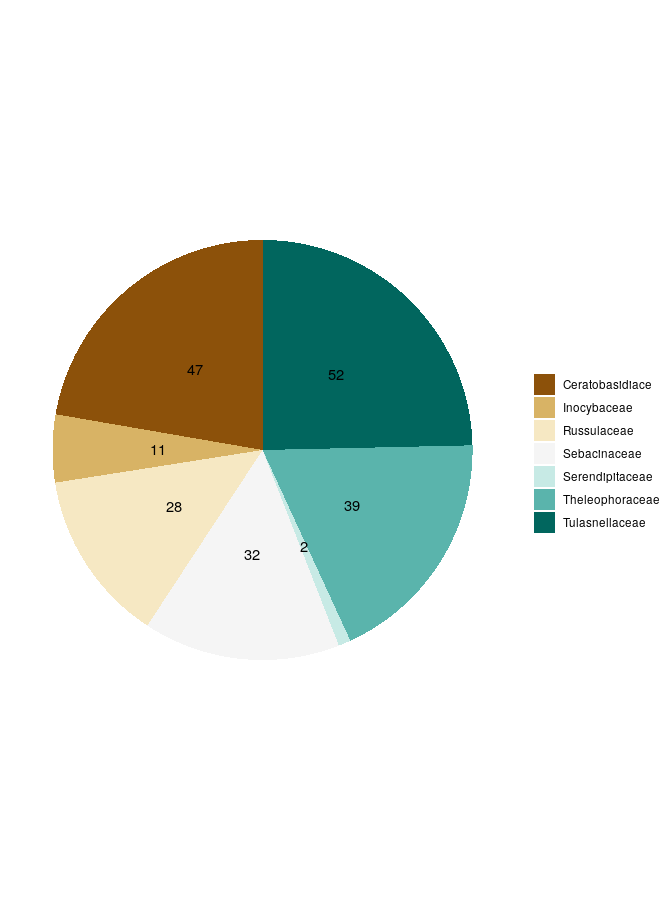
\includegraphics[keepaspectratio,width=\textwidth,height=0.75\textheight]{images/clust.png}
\caption{Number of OTUs from each family}
\end{figure}

\input{latEnd.txt}

\end{document}
